%!TEX root=Principal.tex
\chapter{PROPOSTA}
\label{cap:proposta}

Este trabalho apresenta uma metodologia que mapeia o conjunto de ações que o robô é capaz de executar visando a uma aproximação física do indivíduo, considerando as normas sociais. Como observado ao longo dos trabalhos da literatura apresentados até agora (vide seção~\ref{cap:proxemics}), o comportamento do indivíduo possui dependência da origem ou cultura dele. Assim, algumas reações apresentadas por uma pessoa são diretamente influenciadas pelo seu local de nascimento, pelos locais onde viveu e, consequentemente, pela sua experiência de vida. Contudo, fatores como a experiência de vida e cultura são difíceis de avaliar apenas com a observação.

Dessa forma, essa tese estabelece uma sequência de passos com o intuito de identificar quais são as ações que o robô precisa realizar para que seu comportamento, ao se aproximar de uma pessoa, esteja dentro das normas sociais. A aproximação física é considerado como o primeiro passo para que exista uma interação entre duas pessoas. Com o comportamento adequado do robô nessa aproximação, é possível garantir que uma pessoa fique confortável com a presença física do robô a sua volta. O nível de conforto pode ser medido pela aceitação do robô próximo ao indivíduo por um determinado ciclo de tempo. Essa aceitação, pode determinar o início de uma interação por um período de tempo maior, porém não será abordado esse tipo de interação nessa tese.

O primeiro passo estabelecido é a coleta de variáveis de maneira que não exista, em um primeiro momento, a preocupação do comportamento do robô. Na sequência é aplicado um algoritmo de aprendizado para árvore de decisão, com o objetivo de identificar quais as variáveis mais relevantes para a aproximação do robô. Com as informações sobre as variáveis mais relevantes, é possível utilizar de técnicas para aprendizado de máquina, que faça com que o robô tenha o comportamento adequado com base em pequenas observações sobre a pessoa que ele irá interagir. No final, é possível realizar o perfil das pessoas que interagiram com o robô e identificar qual o comportamento adequado para cada perfil extraído.

Essa seção apresenta em detalhes os passos da metodologia proposta por esta tese. Ao final do capítulo é apresentado a visão completa da metodologia onde é realizado uma síntese do processo como um todo e das técnicas aplicadas nele. Antes de entrar em detalhes na metodologia, é apresentado o robô que será utilizado para o desenvolvimento do estudo proposto nessa tese.

\section{O Robô}
\label{sec:robo}
O robô utilizado no desenvolvimento dessa tese é o PeopleBot~\footnote{PeopleBot - http://www.mobilerobots.com/researchRobots/PeopleBot.aspx} fabricado pela ActivMedia Robotics. Ele é um robô móvel com direção diferencial, ou seja, possui duas rodas motorizadas e uma roda castor que auxilia em seu equilíbrio. O projeto do PeopleBot tem foco em pesquisas e serviços que envolvem interação humano-robô. Com esse objetivo, ele foi desenvolvido com uma altura de 112 cm (centímetros). Além disso, o PeopleBot também possui uma garra pequena que tem sua movimentação apenas na vertical. A figura~\ref{fig:peoplebot} apresenta o robô PeopleBot.

\begin{figure}[ht!]
	\centering
	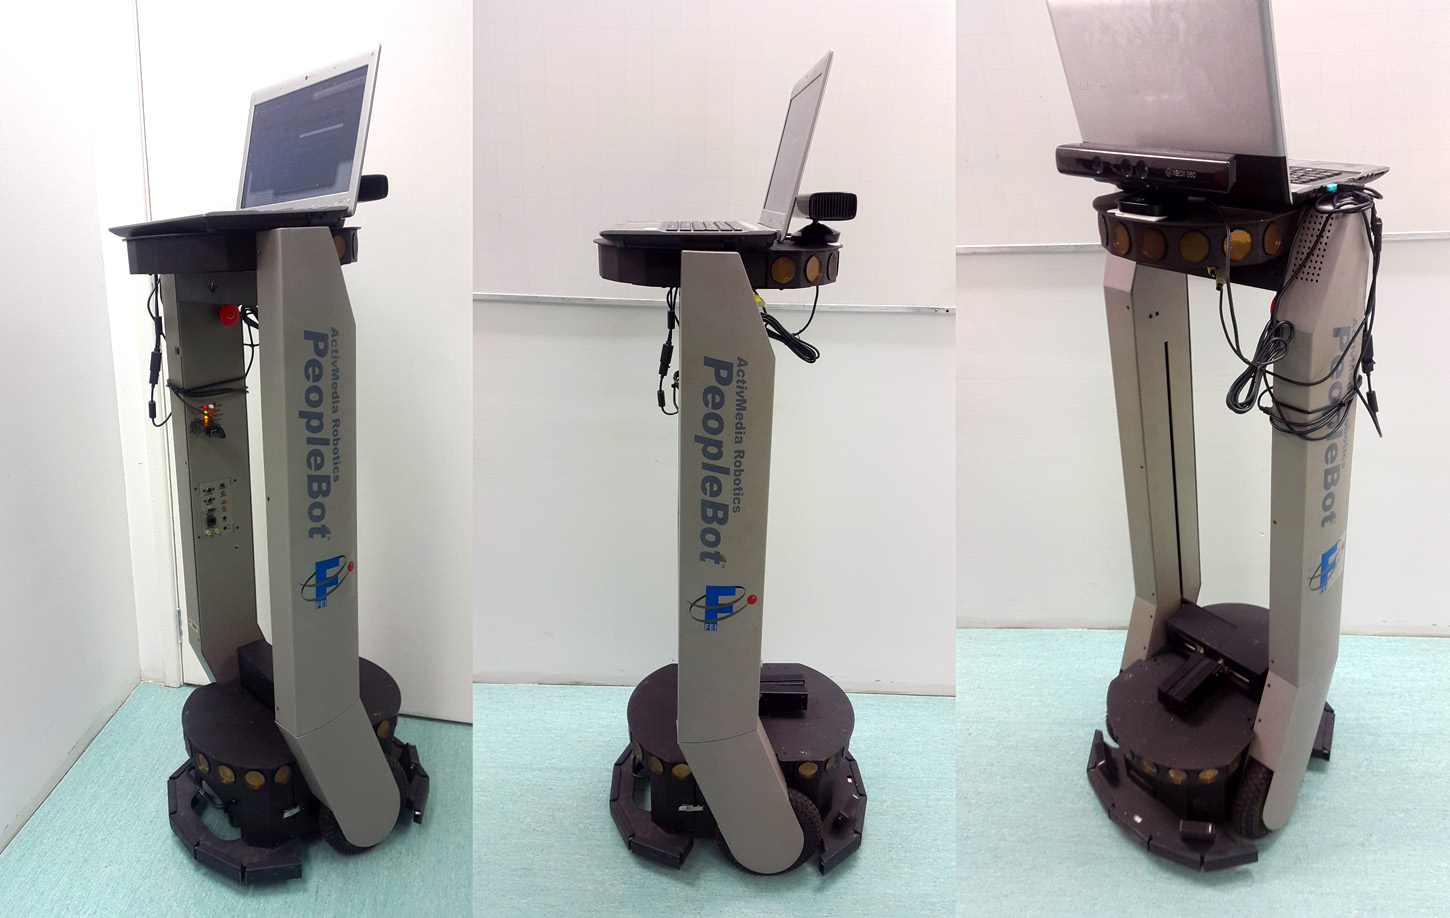
\includegraphics[width=\textwidth]{images/peoplebot.jpg}
	\caption{Robô ActivMedia Robotics PeopleBot.}
	\label{fig:peoplebot}
\end{figure}

Como a garra do PeopleBot é curta e não permite muitos movimentos, foi adicionado um manipulador para auxiliar na manipulação de objetos e gesticulação durante a interação com pessoas e também visando a prestação de serviços domésticos e de cuidados pessoais. O projeto de construção do manipulador é apresentado através da figura~\ref{fig:manipulador}.

\begin{figure}[ht!]
	\centering
	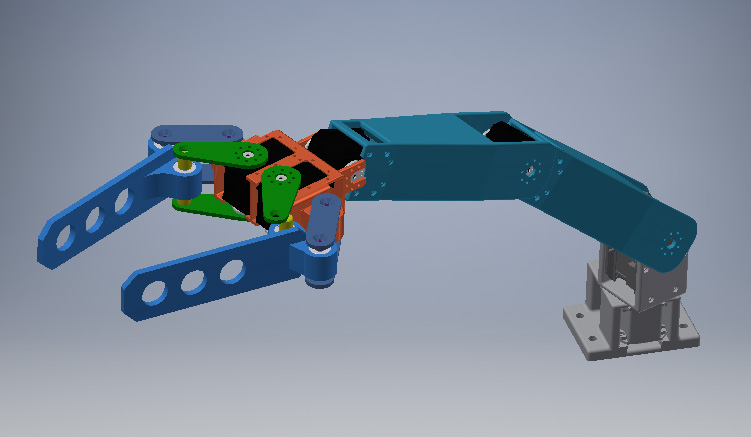
\includegraphics[width=0.6\textwidth]{images/manipulador.jpg}
	\caption{Projeto do Novo Manipulador do PeopleBot.}
	\label{fig:manipulador}
\end{figure}

O novo manipulador foi construído de maneira que os movimentos sejam parecidos com o braço humano. Além do manipulador, também foi acoplado um \emph{tablet} para que seja possível atribuir faces ao robôs e deixar a interação mais amigável, como apresentado na figura~\ref{fig:judithhead}.

\begin{figure}[ht!]
	\centering
	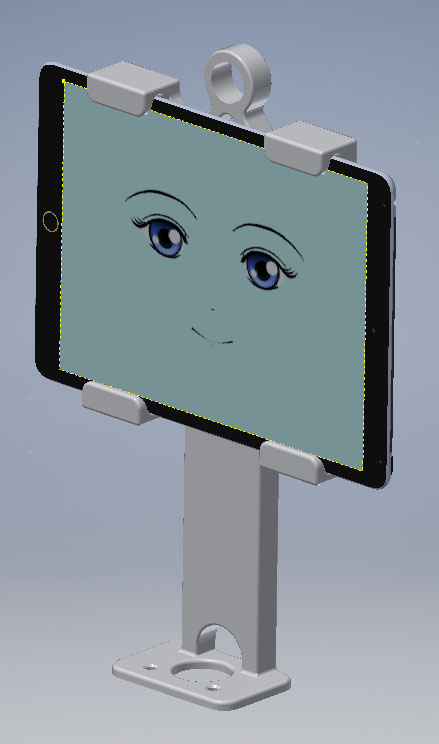
\includegraphics[width=0.4\textwidth]{images/judith_head.jpg}
	\caption{Projeto da Cabeça para o PeopleBot.}
	\label{fig:judithhead}
\end{figure}

Alguns sensores como o Microsoft\textregistered\ Kinect\textregistered\ , o ASUS\textregistered\ Xtion\textregistered\ , lasers e microfones também foram instalados para melhorar a captura das informações que são apresentadas na seção~\ref{sec:extracaocaracteristicas}.

\section{Extração das Características para o RBC}
\label{sec:extracaocaracteristicas}

Como apresentado no capítulo \ref{cap:proxemics}, existem diversas variáveis que podem auxiliar na extração de um perfil comportamental do individuo. \emph{Proxemics} tornam possível a extração de fatores sobre a distância social entre o individuo e o robô. Esses fatores podem variar não só entre a posição física dos dois agentes, mas também na posição do corpo dos indivíduos, como por exemplo, a orientação dos ombros e troco em relação a posição do robô. Outro fator também significante é a fixação entre olhares, este pode determinar o início e o fim de uma interação, além dos principais indivíduos na interação. Além disso, pode ser também empregado o reconhecimento de expressões faciais que auxiliam na análise do quanto a situação é confortável para o individuo, o quanto ele aprecia a interação. Assim, pode existir uma avaliação em tempo real das reações deste durante todo o processo de interação. Outra técnica que pode ser utilizada na análise do conforto do individuo durante a interação é a avaliação da emoção através da voz da pessoa.

Dessa forma, é possível empregar diversos sensores que auxiliam a leitura e quantificação dessas variáveis. Sensores de captura de marcações de movimento, como Microsoft\textregistered\ Kinect\textregistered\ ou o ASUS\textregistered\ Xtion\textregistered, são utilizados para quantificar os valores obtidos através da \emph{Proxemic}, que envolvem distância entre agentes e orientação de membros do individuo. Para realizar o reconhecimento de expressões faciais utiliza-se uma câmera de video, podendo assim executar uma leitura da face do individuo em tempo de execução na interação entre o humano e o robô. As variáveis referentes a questão da fixação dos olhares dos agentes para identificar o início e o fim da interação, podem ser obtidas através de ambos sensores, sendo possível determinar a orientação da cabeça e torso do individuo, além de também a direção do olhar deste para com o robô. A voz do individuo para análise da emoção na interação é obtida através de um microfone. A figura \ref{fig:capturacaracteristicas} apresenta a ilustração do processo de extração das características do individuo.

\begin{figure}[ht!]
	\centering
	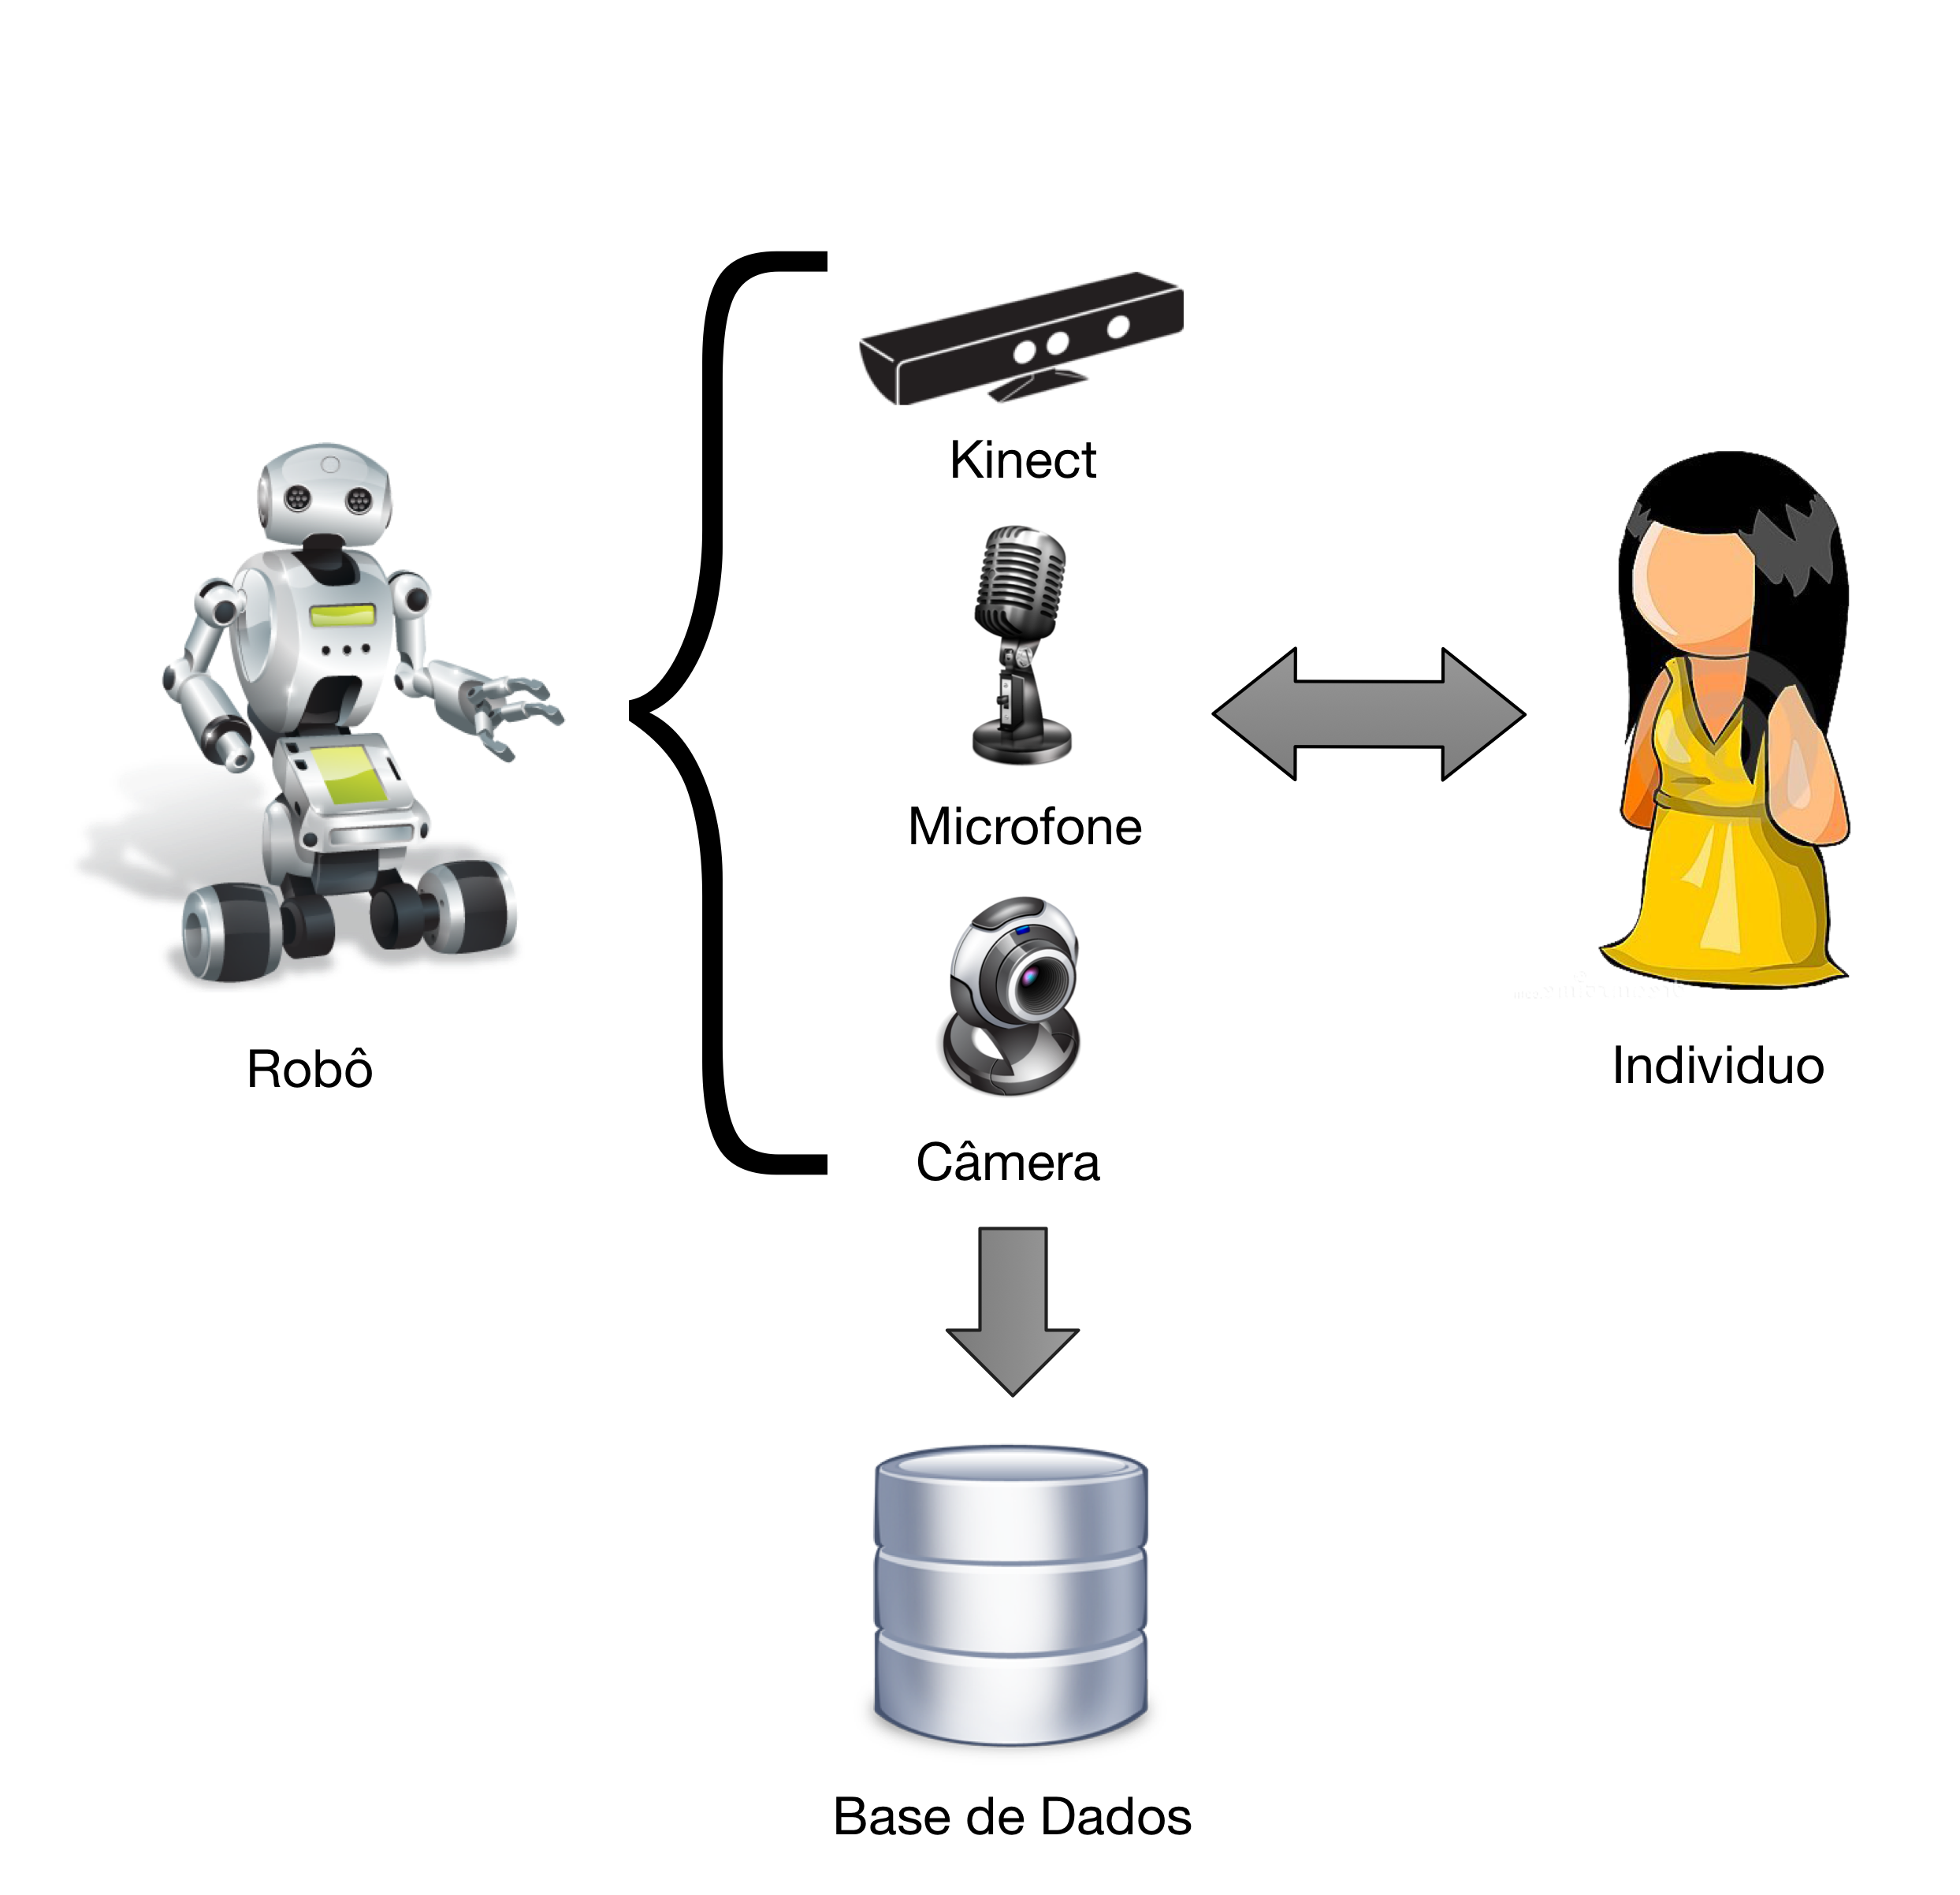
\includegraphics[scale=0.6]{images/captura_carac_individuo.png}
	\caption{Processo para a extração das características do individuo.}
	\label{fig:capturacaracteristicas}
\end{figure}

No processo apresentado pela figura \ref{fig:capturacaracteristicas}, o robô utiliza os sensores para identificar o individuo e iniciar a aproximação dele. Durante a aproximação, o robô utiliza um componente de \emph{log} que armazena todos os valores das variáveis que são utilizadas para determinar, posteriormente, o comportamento do robô (ação) e do individuo (reação) em um banco de dados. As variáveis são apresentadas em detalhes nas seções \ref{sec:variaveisindividuo} e \ref{sec:variaveisrobo}. Com as informações armazenadas é iniciado o processo de aprendizado por árvore de decisão, que auxilia a determinar as variáveis que melhor representam o problema. Além das informações para a árvore de decisão, é possível extrair informações sobre perfis comportamentais das pessoas e identificar com os perfis comportamentais aprendidos pelo robô, para que possa replicar durante a interação. Esse tipo de informação será útil para identificar como é a relação de comportamento entre robôs e humanos. Deve-se lembrar que as informações sobre o comportamento são direcionadas por um cenário de interação, como discutido por \citeonline{Jung:1991} em seu trabalho.

Dessa forma, as variáveis aplicadas ao comportamento tem dependência do cenário de interação, porém as informações das variáveis etnográficas como idade, experiência computacional, sexo, local de origem, etnia, entre outras, são independentes do cenário. Existem alguns algoritmos na área de visão computacional que são capazes de identificar algumas variáveis etnográficas de maneira automática \cite{Yang:2007, Shan:2012, Ylioinas:2012, Samadi:2013, Amaral:2014}, porém para o trabalho desta tese, a coleta dessas informações será realizada através de um questionário pré interação já que esses algoritmos não fazem parte do objetivo principal do trabalho. As informações obtidas através do questionário serão inseridas no banco de dados complementando as informações de comportamento, que são separadas obtidas através da interação entre o ser humano e o robô através dos cenários de interação.

Na seção \ref{sec:variaveisindividuo} são detalhados os conjuntos de variáveis etnográficas e comportamentais com uma breve explicação dos objetivos esperados de cada uma das variáveis coletadas. A seção \ref{sec:variaveisrobo} detalha as variáveis que serão consideradas para o perfil do robô, apresentando também uma explicação sobre os objetivos de cada uma das variáveis.

\subsection{Selecionando as Variáveis para o Individuo}
\label{sec:variaveisindividuo}

Essa seção apresenta os conjuntos de variáveis que são consideradas nesse trabalho como a base de informações para seu desenvolvimento. Dois conjuntos são apresentados, o conjunto de variáveis etnográficas, seguido pelo conjunto de variáveis comportamentais que é o principal foco deste trabalho.

\subsubsection{Conjunto de Variáveis Etnográficas}
\label{sec:variaveisetnograficas}

O objetivo das variáveis etnográficas é identificar qual a experiência social e computacional de cada indivíduo. Além da experiência, também pode-se obter informações sobre a idade, gênero, local de nascimento ou origem do indivíduo. Todas essas informações são relevantes para verificar a existência de uma possível relação entre as variáveis etnográficas e comportamentais. A lista apresentada a seguir define as variáveis etnográficas e uma breve explicação sobre o significado de cada uma das variáveis.

\begin{enumerate}
	\item \textbf{Idade}: informa a idade do indivíduo.
	\item \textbf{Gênero}: informa o sexo biológico do indivíduo.
	\item \textbf{Local de Nascimento}: informa qual o local de nascimento do indivíduo. Essa variável auxiliará a determinar a base cultural do indivíduo.
	\item \textbf{Etnia}: informa a origem da família do indivíduo. Outra variável que auxilia na determinação da base cultural do indivíduo.
	\item \textbf{Quantidade de \emph{Gadgets}}: informa a quantidade de \emph{gadgets} que o indivíduo possui, ajudando a identificar qual a experiência e o contato dele com a tecnologia.
	\item \textbf{Contato prévio com Robôs}: informa apenas se o indivíduo já possuiu algum contato com robôs. Auxiliará a determinar o contato com a tecnologia, principalmente com robôs que poderá influenciar no seu comportamento durante a interação.
	\item \textbf{Tipos de Robôs}: informa quais são os tipos de robôs que o indivíduo teve contato. Os tipos poderão ser robôs \emph{Pet}, Humanoides, Androides, Móveis, entre outros. Essa variável é um complemento da variável ``Contato prévio com Robôs''.
	\item \textbf{Quantidade de cidades visitadas}: informa a quantidade de cidades que o indivíduo já visitou além da sua cidade natal. É importante para identificar o contato com outros tipos de cultura. Isso poderá influenciar no comportamento definido por sua cultura.
	\item \textbf{Quantidade de cidades que morou}: informa a quantidade de cidades que o indivíduo já morou além da sua cidade natal. É importante para identificar a vivência com outros tipos de cultura. Isso poderá influenciar no comportamento definido por sua cultura.
	\item \textbf{Quantidade de países visitadas}: informa a quantidade de países que o indivíduo já visitou além da sua cidade natal. É importante para identificar o contato com outros tipos de cultura. Isso poderá influenciar no comportamento definido por sua cultura.
	\item \textbf{Quantidade de países que morou}: informa a quantidade de países que o indivíduo já morou além da sua cidade natal. É importante para identificar a vivência com outros tipos de cultura. Isso poderá influenciar no comportamento definido por sua cultura.
\end{enumerate}

Em diversos trabalhos da seção \ref{sec:proxemicsihr}, onde a questão cultural do indivíduo é abordada, são discutidos que influência dela sobre o comportamenteo do o indivíduo. Contudo, a cultura é tratada como a origem do indivíduo, por exemplo, no trabalho de \citeonline{Eresha:2013}. Entretanto, a questão cultural na vida de uma pessoa é mais abrangente, está relacionada a experiência adquirida ao longo de sua vivência social. Dessa forma, o conjunto de variáveis apresentado acima tem como objetivo mapear de forma abstrata a experiência social do indivíduo, com o intuito de tornar o comportamento menos dependente da origem e talvez de sua experiência prévia.

Nesse trabalho, as informações levantadas nessa seção serão adquiridas através de questionários pré testes de interação. Em trabalhos futuros serão feitos estudos para identificar essas informações de maneira interativa através do próprio robô.

\subsubsection{Conjunto de Variáveis Comportamentais}
\label{sec:variaveiscomportamentais}

Variáveis comportamentais tem como principal objetivo identificar o comportamento do indivíduo. Nesse trabalho o comportamento está diretamente relacionado com cenários de interação social. As variáveis comportamentais são coletadas a partir de informações sobre as posições corporais e expressões faciais do indivíduo, tornando possível uma análise com base em teorias de linguagem corporal. As análises realizadas a partir da linguagem corporal, tem por base o trabalho apresentado por \citeonline{Lambert:2008}. O conjunto de variáveis comportamentais apresentados nessa seção não são utilizadas apenas para extrair o perfil do indivíduo, mas também para avaliar se a ação realizada pelo robô gerou uma reação positiva ou negativa no indivíduo. A lista apresentada a seguir define as variáveis comportamentais e uma breve explicação sobre o objetivo de cada uma das variáveis.

\begin{enumerate}
	\item \textbf{Expressões Faciais}: é possível identificar se a reação do indivíduo foi positiva ou negativa, a partir de uma ação do robô. Existem seis expressões bases que combinadas formam diversas outras~\cite{Bihan:2014}. Contudo, nesse trabalho será considerado apenas as seis expressões bases classificadas em dois grupos: expressões faciais positivas e expressões faciais negativas. O intuito dessa variável é realizar a avaliação da ação do robô com base nas expressões faciais do indivíduo.
	\item \textbf{Tempo de Transição entre as Zonas Sociais}: identificar o tempo que o indivíduo ficou confortável com a presença do robô a medida que esse diminuiu a distância entre eles.
	\item \textbf{Frequência do Olhar em direção ao Robô}: identificar se o indivíduo mantém o olhar ao robô, sendo possível saber se a interação está continua ou não. Isso pode influenciar se o robô está interagindo de maneira confortável ao indivíduo ou se esse está incomodado com a presença do robô.
	\item \textbf{Tempo do Olhar}: é possível mensurar o interesse do indivíduo durante a interação através do tempo que ele permanece com o olhar fixo no robô. Quanto maior o tempo do olhar, maior o interesse na interação do indivíduo.
	\item \textbf{Orientação dos ombros}: Auxilia a mensurar o interesse do indivíduo durante a interação, analisando se os ombros possuem a mesma orientação que a cabeça e também uma orientação em direção ao indivíduo que interage com o robô. Além disso, é possível determinar através do alinhamento do quadril com o ombro do indivíduo o ângulo de inclinação de seu torso. A inclinação do torso auxilia a identificar o interesse do indivíduo na interação, para isso basta verificar se ele está inclinado em direção ao robô para determinar um interesse positivo.
	\item \textbf{Orientação do quadril}: Auxilia a mensurar o interesse do indivíduo durante a interação. A orientação do quadril em direção ao robô ou na direção oposta auxilia a determinar o grau de interesse do indivíduo na interação. Quando mais alinhado à direção do robô, maior o interesse do indivíduo na interação.
	\item \textbf{Estilo da Voz}: é importante, pois pode determinar a reação que o indivíduo terá após a interação via áudio com o robô. Além disso, é possível determinar se o indivíduo está confortável ou não durante a interação, analisando o tom de sua voz ao responder o robô. Nesse trabalho, será considerado somente o canal de resposta ao indivíduo. A análise do tom da voz do indivíduo não será considerado nesta tese e ficará para trabalhos futuros de aprimoramento do componente de análise comportamental em IHR.
\end{enumerate}

\subsection{Selecionando as Variáveis para o Robô}
\label{sec:variaveisrobo}
Além das variáveis referentes ao perfil do indivíduo, deve-se considerar também as informações sobre o robô uma vez que sua aparência pode influenciar na reação das pessoas durante a interação~\cite{Hegel:2009}. Coletar as variáveis do robô pode auxiliar a identificar quais são os principais fatores que tornam a interação humano-robô desconfortável ou com menos qualidade. Dessa forma, foi definido um conjunto de variáveis que pudessem caracterizar da melhor maneira fatores do robô, referente a sua aparência, que influenciam na IHR. Esse conjunto de variáveis é apresentado a seguir:

\begin{enumerate}
	\item \textbf{Altura}: A altura do robô para identificar a influência da diferença entre alturas de robôs e humanos.
	\item \textbf{Volume}: O volume ocupado pelo robô pode influenciar no conforto da interação, uma vez que quando o robô atingir uma zona social mais próxima do indivíduo pode causar uma sensação claustrofóbica a ele.
	\item \textbf{Tipo do Robô}: Segundo \citeonline{Choi:2014}, robôs possuem dois tipos: Autônomos e Tele-operados. Essa variável define o quanto de intervenção humana é necessário para que o robô possa executar a tarefa objetivo.
	\item \textbf{Classificação do Robô}: Segundo \citeonline{Dobra:2014} classificar um robô é uma tarefa muito complexa e pode envolver diversas variáveis. Dessa forma, para essa tese será considerado uma classificação mais simples. O robô deve ser classificado como: fixo, móvel com rodas, móvel bípede, móvel quadrupede, móvel com manipuladores. Outras classificações podem ser inseridas conforme a necessidade e inclusão de novos robôs.
	\item \textbf{Aparência Física}: Essa variável descreve se o robô possui uma aparência amigável ou agressiva.
	\item \textbf{Nível de Ruído}: Determina qual o nível de ruído que os atuadores do robô podem gerar de tal forma, que possa influenciar na interação humano-robô.
\end{enumerate}

Além das variáveis que definem as características, é necessário também o mapeamento das ações que o robô irá executar para que exista uma avaliação dessa após a reação do indivíduo. As variáveis que compõem as informações do perfil comportamental do robô são:

\begin{enumerate}
	\item \textbf{Aproximação}: Forma de aproximação do robô ao indivíduo. Pode ser classificada entre rápida, devagar, brusca ou suave.
	\item \textbf{Movimentação do Manipulador}: Caso exista um manipulador deve descrever como é feita a movimentação do manipulador em direção ao usuário. A classificação consiste em brusca ou suave.
	\item \textbf{Estilo de Voz}: Ao emitir algum tipo de som o robô deverá manter um estilo de voz para que seja possível simbolizar qual o tipo de mensagem ele deseja falar. A classificação será feita de maneira simplificada, considerando apenas se é um estilo educado ou agressivo.
	\item \textbf{Expressão Facial}: Ao iniciar o contato visual com o indivíduo, pode ocorrer diversas expressões do robô na tentativa de manter o conforto do indivíduo durante o processo de interação. Simplificando as expressões, de maneira similar ao apresentado na seção~\ref{sec:variaveiscomportamentais}, são consideradas apenas dois tipos de expressões realizadas pelo robô: amistoso e não-amistoso. As expressões faciais do robô serão executadas através do \emph{tablet} acoplado nele, conforme descrito na seção~\ref{sec:robo}.
\end{enumerate}

As variáveis comportamentais do robô definidas com o objetivo de executar uma tarefa de abordagem para estabelecer uma interação. Caso seja necessário adicionar novas variáveis a esse conjunto não haverá problema ao método apresentado ao longo da seção.

\section{Identificando a relevância das variáveis}
\label{sec:decisiontree}

Aqui será descrito todo o processo para gerar a árvore de decisão.

\begin{figure}[ht!]
	\centering
	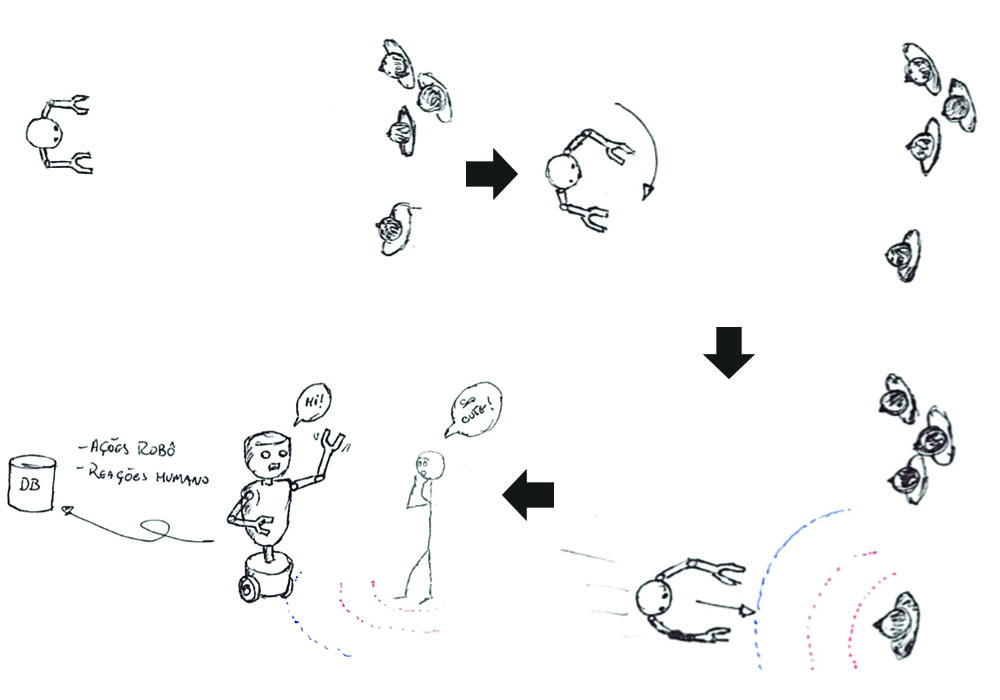
\includegraphics[width=\textwidth]{images/decision_tree_process.jpg}
	\caption{Processo de Interação para Gerar a Árvore de Decisão.}
	\label{fig:rbc}
\end{figure}
